% !TEX encoding = UTF-8
% !TEX TS-program = pdflatex
% !TEX root = ../tesi.tex

%**************************************************************
\chapter{Progetto di stage}
\label{cap:progetto-stage}
%**************************************************************

\section{Analisi dei requisiti}

Prima di iniziare a lavorare sul progetto, il tutor aziendale, mi ha fornito la documentazione esistente dell'applicativo, in particolar modo ho fatto riferimeto al manule
utente creato in precedenza e all'analisi dei requisiti. Mi è stato espressamente chiesto inoltre di non eseguire alcuna modifica a livello grafico dell'applicativo in quanto 
la clientela era abituata alla versione corrente e non sempre è immediato addattarsi a cambiamenti di questo tipo.
Ho infine aggiunto due casi particolari che verranno evidenziati di seguito per quanto riguarda l'analisi dei requisiti esistente.

%************************************************************

\subsection{Casi d'uso}

Per rappresentare l'insieme delle azioni comuni ad un singolo utente sono stati utilizzati i casi d'uso.
Per descrivere i vari scenari ho mantenuto la precedente scaletta di informazioni così da dare una continuità al documento esistente. 
Ciascun caso d'uso sarà quindi rappresentato come descritto di seguito:
\begin{itemize}
    \item \textbf{Identificatore} univo nel formato UC-[Codice];
    \item \textbf{Titolo} del caso d'uso;
    \item \textbf{Descrizione} generale del caso d'uso;
    \item \textbf{Attori} coinvolti: primari e secondari;
    \item \textbf{Precondizione} del caso d'uso;
    \item \textbf{Scenario principale} che il caso d'uso vuole modellare, identificando ogni azione che ne fa parte;
    \item \textbf{Postcondizione} del caso d'uso;
    \item \textbf{Estenzioni} dello scenario principale, evidenziata da una lettera maiuscola e inserita in un elenco.
\end{itemize}

Di seguito vengono rappresentate le modifiche apportate al documento esistente.
Si fa riferimento allo standard UML 2.0 per la rappresentazione dei casi d'uso.

\subsection*{UC-3 Pianificazione della produzione}

\begin{figure}[H]
	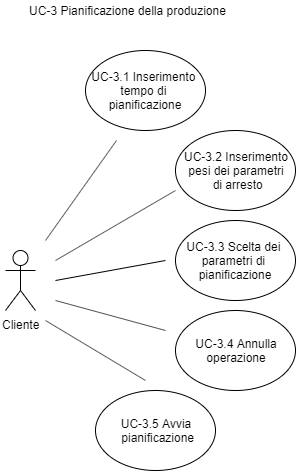
\includegraphics[width=8cm]{immagini/UC1.png}
	\centering
	\caption{Use Case - UC-3}
\end{figure}

\textbf{Attori}: Cliente. \newline
\textbf{Descrizione}: Il cliente esegue la pianificazione degli ordini selezionati.\newline
\textbf{Precondizione}: Il cliente ha selezionato gli ordini che intende pianificare e i giorni in cui vuole farlo.\newline
\textbf{Scenario principale}: \begin{itemize}
    \item Il cliente seleziona che ordini vuole pianificare;
    \item Il cliente preme il pulsante "Pianifica";
    \item Il cliente modifica i parametri della pianificazione come previsto dagli UC-3.1, UC-3.2, UC-3.3;
    \item Il cliente preme il pulsante "Avvia pianificazione".
\end{itemize}

\textbf{Postcondizione}: Nella finestra principale viene visualizzato il risultato della pianificazione.


\subsection*{UC-3.3 Scelta dei parametri di pianificazione}

\begin{figure}[H]
	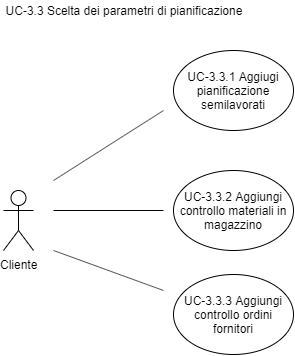
\includegraphics[width=8cm]{immagini/UC2.png}
	\centering
	\caption{Use Case - UC-3.3}
\end{figure}

\textbf{Attori}: Cliente. \newline
\textbf{Descrizione}: Il cliente seglie i parametri da considerare nella pianificazione.\newline
\textbf{Precondizione}: Il cliente ha selezionato il pulsante "Metodo di pianificazione".\newline
\textbf{Scenario principale}: \begin{itemize}
    \item Il cliente seleziona come effettuare le pianificazione;
    \item Il cliente può selezionare le varie aggiunte descritte dagli UC-3.3.1, UC-3.3.2, UC3.3.3;
    \item Il cliente preme il pulsante "Conferma".
\end{itemize}
\textbf{Postcondizione}: Si verrà ricondotti allo use case UC-3.3.
\newpage
\section{Tracciamento dei requisiti}

Ogni requisito è composto dalla seguente struttura:
\begin{itemize}
	\item \textbf{codice identificativo}: ogni codice identificativo è univoco e conforme alla seguente codifica:\\
	\centerline{\textbf{R[Importanza][Tipologia][Codice]}} \\ \\
	Il significato delle cui voci è:
	\begin{itemize}
		\item \textbf{Tipologia}: ogni requisito può assumere uno dei seguenti valori:
		\begin{itemize}
			\item \textit{F}: funzionale;
			\item \textit{P}: prestazionale;
			\item \textit{Q}: qualitativo;
			\item \textit{V}: vincolo.
		\end{itemize}
		\item \textbf{Importanza}: ogni requisito può assumere uno dei seguenti valori:
		\begin{itemize}
			\item \textit{O}: requisito obbligatorio: irrinunciabili per qualcuno degli stakeholder;
			\item \textit{D}: requisito desiderabile: non strettamente necessari ma  a valore aggiunto riconoscibile;
			\item \textit{F}: requisito facoltativo: relativamente utili oppure contrattabili più avanti nel progetto.	
		\end{itemize}
		\item \textbf{Codice}: è un identificatore univoco del requisito segue un ordine incrementale.
	\end{itemize}
	\item \textbf{classificazione}: viene riportata l'importanza del requisito. Sebbene questa sia un'informazione ridondante ne facilita la lettura;
	\item \textbf{descrizione}: descrizione breve ma completa del requisito, meno ambigua possibile.
\end{itemize}
\renewcommand{\arraystretch}{1.5}



\subsection{Requisiti funzionali}


\renewcommand{\arraystretch}{1.5}
\rowcolors{2}{dispari}{pari}
\arrayrulecolor{white}

\begin{longtable}{ >{\centering}p{0.15\textwidth} >{\centering}p{0.20\textwidth}
		>{\raggedright}p{0.35\textwidth} >{\centering}p{0.14\textwidth}}
	\caption{Tabella dei requisiti funzionali}\\
	\rowcolorhead 
	\textbf{\color{white}Requisito} 
	& \textbf{\color{white}Classificazione} 
	& \centering\textbf{\color{white}Descrizione}
	 
	\endfirsthead
	\rowcolor{white}\caption[]{(continua)}\\
	\rowcolorhead 
	\textbf{\color{white}Requisito} 
	& \textbf{\color{white}Classificazione} 
	& \centering\textbf{\color{white}Descrizione}
	
	\endhead	
	
	RFO1	&	Obbligatorio	&	Il sistema permette l’inserimento di un nuovo vincolo di linea	 \tabularnewline
	RFO2	&	Obbligatorio	&	Il sistema permette la modifica dei dati di un vincolo di linea esistente	\tabularnewline
	RFO3	&	Obbligatorio	&	Il sistema permette l’eliminazione di un vincolo di linea 	\tabularnewline
	RFO4	&	Obbligatorio	&	L’interfaccia permette l’eliminazione di una linea 	\tabularnewline
	RFO5	&	Obbligatorio	&	 Il sistema permette l’aggiunta di una nuova sequenza	\tabularnewline
	RFO6	&	Obbligatorio	&	 Il sistema permette la modifica dei dati di una sequenza esistente	\tabularnewline
	RFO7	&	Obbligatorio	&	 Il sistema permette l’eliminazione di un articolo di sequenza esistente	\tabularnewline
	RFO8	&	Obbligatorio	&	 Il sistema permette l’eliminazione di un vincolo di sequenza esistente	\tabularnewline
	RFO9	&	Obbligatorio	&	 Il sistema permette l’eliminazione di una sequenza	\tabularnewline
	RFO10	&	Obbligatorio	&	 Il sistema permette all’utente di scegliere un tempo massimo di esecuzione dell’algoritmo	\tabularnewline
	RFO11	&	Obbligatorio	&	 Il sistema permette all’utente di assegnare un peso all’importanza di parametri di produzione quali:pezzi prodotti e occupazione delle linee	\tabularnewline
	RFD1	&	Desiderabile	&	 Il sistema permette all’utente di scegliere se ricalcolare la pianificazione già esistente	\tabularnewline
	RFO12	&	Obbligatorio	&	 Il sistema permette di pianificare automaticamente la produzione dato un insieme di ordini e un intervallo di tempo	\tabularnewline
	RFO1	&	Obbligatorio	&	 Il sistema permette di scegliere i relativi criteri di pianificazione	\tabularnewline
\end{longtable}

\newpage
\subsection{Requisiti qualitativi}

\rowcolors{2}{pari}{dispari}

\begin{longtable}{ >{\centering}p{0.15\textwidth} >{\centering}p{0.20\textwidth}
		>{\raggedright}p{0.35\textwidth} >{\centering}p{0.14\textwidth}}
	\caption{Tabella dei requisiti qualitativi}\\
	\rowcolorhead 
	\textbf{\color{white}Requisito} 
	& \textbf{\color{white}Classificazione} 
	& \centering\textbf{\color{white}Descrizione}
	 
	\endfirsthead
	\rowcolor{white}\caption[]{(continua)}\\
	\rowcolorhead 
	\textbf{\color{white}Requisito} 
	& \textbf{\color{white}Classificazione} 
	& \centering\textbf{\color{white}Descrizione}
	
	\endhead	
	
	RQD1	&	Desiderabile	&	Il programma genera un file di Log\glosp di supporto al Debug\glo	 \tabularnewline
	RQO1	&	Obbligatorio	&	Ogni scelta non banale effettuata è adeguatamente commentata nel codice	\tabularnewline
	RQF1	&	Facoltativo		&	Fornire un manuale utente	\tabularnewline
	RQF2	&	Facoltativo		&	Fornire un manuale sviluppatore	\tabularnewline

\end{longtable}

\subsection{Requisiti prestazionali}

\rowcolors{2}{pari}{dispari}

\begin{longtable}{ >{\centering}p{0.15\textwidth} >{\centering}p{0.20\textwidth}
		>{\raggedright}p{0.35\textwidth} >{\centering}p{0.14\textwidth}}
	\caption{Tabella dei requisiti prestazionali}\\
	\rowcolorhead 
	\textbf{\color{white}Requisito} 
	& \textbf{\color{white}Classificazione} 
	& \centering\textbf{\color{white}Descrizione}
	 
	\endfirsthead
	\rowcolor{white}\caption[]{(continua)}\\
	\rowcolorhead 
	\textbf{\color{white}Requisito} 
	& \textbf{\color{white}Classificazione} 
	& \centering\textbf{\color{white}Descrizione}
	
	\endhead	
	
	RPD1	&	Desiderabile	&	L'applicativo deve fornire una soluzione entro il tempo stabilito dall'utente	 \tabularnewline
	RPD2	&	Desiderabile	&	L'applicativo deve fornire la soluzione nel modo più rapido possibile senza valutare ulteriori combinazioni se è stato
	raggiunto un determinato punteggio stabilito per la soluzione stessa \tabularnewline
	RPD3	&	Desiderabile	&	La fase di lettura dei dati deve essere eseguita in tempi inferiori ai 30 minuti \tabularnewline

\end{longtable}
\newpage
\subsection{Requisiti vincolo}

\rowcolors{2}{pari}{dispari}

\begin{longtable}{ >{\centering}p{0.15\textwidth} >{\centering}p{0.20\textwidth}
		>{\raggedright}p{0.35\textwidth} >{\centering}p{0.14\textwidth}}
	\caption{Tabella dei requisiti prestazionali}\\
	\rowcolorhead 
	\textbf{\color{white}Requisito} 
	& \textbf{\color{white}Classificazione} 
	& \centering\textbf{\color{white}Descrizione}
	 
	\endfirsthead
	\rowcolor{white}\caption[]{(continua)}\\
	\rowcolorhead 
	\textbf{\color{white}Requisito} 
	& \textbf{\color{white}Classificazione} 
	& \centering\textbf{\color{white}Descrizione}
	
	\endhead	
	
	RVO1	&	Desiderabile	&    Rendere compatibile il programma con l’attualemodulo di pianificazione della produzione	 \tabularnewline
	RVO2	&	Desiderabile	&    Ottimizzare la pianificazione tenendo conto delle materie prime e dei semilavorati	 \tabularnewline
	RVO3	&	Desiderabile	&    Ottimizzare la pianificazione tenendo conto degli ordini dei fornitori inseriti a sistema	 \tabularnewline
	RVO4	&	Desiderabile	&    Ottimizzare la pianificazione rendendo possibile la pianificazione dei semilavorati	 \tabularnewline
	RVO5	&	Desiderabile	&    Il programma è sviluppato tramite il linguaggio diprogrammazione Vb.NET v.4.7.0	 \tabularnewline
	RVO6	&	Desiderabile	&    L’IDE\glosp utilizzato è Microsoft Visual Studio\glosp v.10.0.4	 \tabularnewline
	RVO7	&	Desiderabile	&    Le componenti grafiche sono basate sulle DevEx-press\glo	 \tabularnewline
	RVO8	&	Desiderabile	&    I dati vengono salvati su un database Informix	 \tabularnewline
	RVO9	&	Desiderabile	&    I dati in input sono scritti su un file JSON	 \tabularnewline
	RVO10	&	Desiderabile	&    I dati in output sono scritti su un file JSON	 \tabularnewline

\end{longtable}

\newpage
\subsection{Riepilogo dei requisiti}

\rowcolors{2}{pari}{dispari}

\begin{longtable}{ >{\centering}p{0.15\textwidth} >{\centering}p{0.20\textwidth}
		>{\raggedright}p{0.35\textwidth} >{\centering}p{0.14\textwidth}}
	\caption{Tabella del riepilogo dei requisiti}\\
	\rowcolorhead 
	\textbf{\color{white}Tipo} 
	& \textbf{\color{white}Obbligatori} 
	& \centering\textbf{\color{white}Desiderabili}
	& \centering\textbf{\color{white}Facoltativi}
	
	\endhead	
	
	Funzionali	&	13	&  1  &	0 \tabularnewline
	Qualitativi	&	1	&  1  &	 2 \tabularnewline
	Prestazionali	&	0	&   3 & 0	 \tabularnewline
	Di vincolo	&	10	& 0   &	0 \tabularnewline
	Totali	&	24	&   5 &	2 \tabularnewline
\tabularnewline \tabularnewline
\end{longtable}
\newpage
\section{Tecnologie e strumenti}

Di seguito sono riportate tutte le tecnologie utilizzate durante lo sviluppo del progetto.
Tali scelte sono state imposte da Ergon Informatica in quanto sono gli strumenti che vengono utilizzati dall'azienda per lo sviluppo dei progetti interni.
La scelta è inoltre guidata dal fatto che, per mantenere l'integrazione con le parti già esistenti dell'applicativo e il suo funzionamento tramite il software Ergdis, 
non si è potuto spostarsi su nuove tecnologie, magari anche solo a qualche versione successiva di esse.
Ergon Informatica si appoggia a questi strumenti in quanto sono forniti di un ottima documentazione di supporto, hanno un alto tasso di scalabilità 
e forniscono un supporto in tempo reale alla codifica.\\ \\

\textbf{Vb.NET}

\begin{figure}[H]
	
\includegraphics[width=5cm]{immagini/vb.png}
	\centering
	\caption{Logo Vb.NET}
\end{figure}

Linguaggio di programmazione che deriva da Visual Basic 6, è sviluppato da Microsoft e, al contrario dei precedenti, supporta il paradigma di programmazione orientata agli oggetti.
Vb.NET consente lo sviluppo di applicazioni Windows, Web e per dispositivi mobili. 
Come avviene con tutti i linguaggi basati su Microsoft .NET Framework,
i programmi scritti in Vb.NET usufruiscono delle funzionalità di sicurezza e interoperabilità dei linguaggi.
Nel progetto viene utilizzato questo linguaggio per poter usufruire delle classi, le quali riducono significativamente le duplicazioni di codice e rendono l'intero sorgente 
chiuso alle modifiche e aperto agli ampliamenti. Viene inoltre utilizzato in quanto è il linguaggio attualmente adottato dall'azienda per lo sviluppo e si presta bene
al tipo di lavorazioni necessarie a portare a compimento lo sviluppo dell'applicativo.

\newpage
\textbf{Visual Studio 2010}

\begin{figure}[H]
	
\includegraphics[width=9cm]{immagini/microsoft-visual-studio-2010-logo.png}
	\centering
	\caption{Logo Visuali Studio 2010}
\end{figure}

Ambiente di sviluppo integrato sviluppato da Microsoft. 
La prima versione risale al 1997 e aveva lo scopo di fornire
un ambiente di sviluppo grafico ed  ed integrato che aiutasse lo sviluppatore a gestire i progetti in maniera semplice, ma efficace, aumentandone quindi la produttività.
Microsoft ha incluso il supporto a differenti linguaggi di programmazione.
In Ergon Informatica è il principale ambiente di sviluppo sia per applicazioni desktop che mobile, di conseguenza è stato utilizzato anche durante lo sviluppo del progetto.\\

\textbf{DevExpress}

\begin{figure}[H]
	\includegraphics[width=8cm]{immagini/devexpress.png}
	\centering
	\caption{Logo DevExpress}
\end{figure}

\textit{Developer Express Inc.} è una società di sviluppo software fondata nel 1998, inizialmente fornisce un insieme di controlli UI\glosp poi sviluppa diverse estensioni per le librerie grafiche.
In particolare nel progetto ci si è appoggiati a questa tecnologia per velocizzare la creazione dell'interfaccia grafica sulla quale si basa il modo di rappresentare la soluzione
che viene fornita, permettendo una chiara visualizzazione tabellare grazie ad una delle tante estensioni\glosp utilizzabili. 

\newpage
\textbf{JSON}

\begin{figure}[H]
	
\includegraphics[width=3cm]{immagini/json.png}
	\centering
	\caption{Logo JSON}
\end{figure}

Acronimo di \textit{JavaScript Object Notation}, è un formato adatto all'interscambio di dati fra applicazioni client/server\glo.
Serve, in particolare, a fornire una struttura a dati interessati rendendoli interscambiabili tra diverse applicazioni senza che si renda necessaria la codifica e decodifica di quest'ultimi.
Nel nostro caso si rende utile quando è necessario delegare l'esecuzione di operazioni sui dati prelavati da un terminale con accesso al database verso un terminale esterno.
I dati raccolti dal database venivano trasferiti in un file JSON, il quale veniva inviato al successivo passo di esecuzione dell'algoritmo, al termine di ciò veniva restituita
la soluzione sempre in formato JSON a chi ne aveva fatto richiesta e di conseguenza visualizzata.\\

\textbf{Informix}

\begin{figure}[H]
	\includegraphics[width=7cm]{immagini/Informix.png}
	\centering
	\caption{Logo Informix}
\end{figure}

Fa parte della divisione DBMS\glosp di IBM\glosp, è un sistema software progettato per consentire la creazione, la manipolazione e l'interrogazione efficiente di database.
L'Informix server supporta il modello relazionale ad oggetti che permette ad IBM di offrire estensioni che supportano i tipi di dati che non sono una parte dello standard SQL\glo.
Le estensioni più usate sono quelle riguardanti le serie temporali e spaziale che forniscono entrambe supporto al tipo di dato ed estensioni linguistiche che permettono 
interrogazioni per un dominio specifico ad alte prestazioni e archiviazione efficiente per set di dati basati su serie temporali e dati spaziali.
È il servizio database sul quale fa affidamento l'azienda essendo anche uno dei partner principali.